% Software
\specialsection{Software}{}{black}{white}
\subsection{Editor}
\subsection{Releases}
\subsection{A cathedral or a bazaar}

While existing literature often focuses on the role of companies in contributing to open-source projects through complementary services like consulting, our study diverges by focusing on individual contributors. In the context of the Processing community, corporate involvement is notably lesser when compared to platforms like Linux that have substantial corporate contributions.

The 2016 Processing community survey revealed a significant number of users employ the language for educational purposes. This is consistent with Processing's design ethos, which is aimed at being educationally accessible. However, the extent to which this educational usage intersects with what can be termed as `professional use' remains unclear.

For the purpose of this study, `professional use' is understood to primarily include artists and designers. This nuanced categorization helps in probing the overlap between professional and educational use within the Processing community.

Building upon established frameworks such as the taxonomy by Bonaccorsi et al.~\cite{bonaccorsiComparingMotivationsIndividual2006}, which categorizes motivations behind open-source contributions into Economic, Social, and Technological domains, our study intends to adapt this taxonomy to suit the specific nuances of the Processing community.

\begin{figure}[h!] 
  \centering
  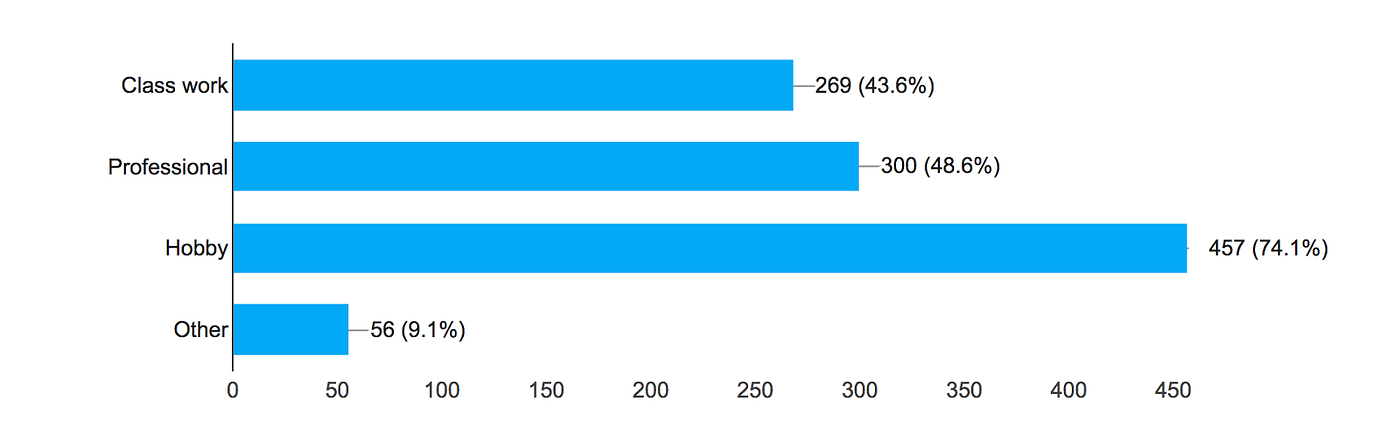
\includegraphics[width=0.9\textwidth]{images/community-survey.png} 
  \caption{Processing 2016 community survey result \parencite{2016CommunitySurvey}}
  \label{fig:community_survey}
\end{figure}

\begin{table}
    \begin{tabularx}{\textwidth}{l X} % X is a placeholder for stretching the column
    \toprule
    Motivation area & Micro level \\
    \midrule
    Economic & Monetary rewards \\
     & Low opportunity costs \\
     & Gaining a reputation among peers \\
     & Gaining future career benefits \\
    \midrule
    Social & Fun to program (Loving to code) \\
     & Altruism (gift economy) \\
     & Sense of belonging to the community \\
     & Fight against proprietary software \\
    \midrule
    Technological & Learning \\
     & Contributions and feedback from the community \\
     & Working with a bleeding-edge technology \\
     & Scratching a personal itch \\
    \bottomrule
    \end{tabularx} % End of tabularx environment
    \label{tab:taxonomy}
    \caption{Taxonomy of Individual Programmers’ Motivations. Adapted from \parencite{bonaccorsiComparingMotivationsIndividual2006}}

\end{table}

% todo NN cette taxonomie est intéressante, mais il faudrait la commenter dans le corps de texte en 2.2, qu’elle vienne nourrir ce que tu as mis au-dessus comme texte, là tu la pose rapidement sans trop détailler comment elle a été produite et ce qu’elle nous dit

%\subsection{The intersection of Creative Coding and Open Source}
%\subsection{Relevant Methodological Approaches in Computer Science and Anthropology}

\subsection{Open Source Contributions}

Open source software has evolved from a grassroots, community-driven activity into a mainstream phenomenon influencing all sectors of software development. This transition has been analyzed from numerous perspectives, including Etienne Wenger's theory of Communities of Practice, which posits that learning occurs in social contexts \parencite{wengerCommunitiesPracticeLearning1998}. This theory underscores the importance of shared experiences, tools, and discourse in shaping a community's collective practice. In the context of open-source software, these dynamics offer invaluable insights into the sustainability and progression of such projects. For instance, the Processing community exemplifies more than just a collection of individual contributors; it represents a dynamic community molded by common goals and collective learning.

This communal focus contrasts sharply with the software development models described in Eric S. Raymond's seminal work "The Cathedral and the Bazaar" \parencite{CathedralBazaarMusings2002a}. The Cathedral model is marked by careful planning and centralized authority, more akin to the early GNU projects initiated by Richard Stallman in the 1980s. Conversely, the Bazaar model encourages open collaboration and decentralization—features commonly associated with contemporary open source projects. These two models can be conceptualized as endpoints of a continuum, with real-world communities of practice, like the Processing community, potentially embodying characteristics of both.

Although Richard Stallman's Free Software Movement initially utilized a Cathedral-like approach, the evolution of version control systems like Git has facilitated the adoption of more decentralized, Bazaar-like models. This technological and philosophical shift intriguingly complements Wenger's notions of "mutual engagement," "joint enterprise," and "shared repertoire"—elements that nurture a sense of community and shared objectives \parencite{wengerCommunitiesPracticeLearning1998}.

Fast-forwarding to today, the landscape now includes not just individual contributors but major corporations as well, injecting both challenges and opportunities into existing communities. The Processing project stands as a compelling case study to examine how an open-source community can preserve its foundational ethos while simultaneously adapting to contemporary requirements.

To holistically grasp the intricate interplay of social and technical factors contributing to the success of open-source initiatives, a multidimensional analysis is essential. Such an approach would synthesize various frameworks, including Wenger's Communities of Practice \parencite{wengerCommunitiesPracticeLearning1998} and Raymond's Cathedral and Bazaar models \parencite{CathedralBazaarMusings2002a}, aiming to provide a nuanced understanding of a community's past, present dynamics, and future potential.

